Para el sistema del problema anterior, si
\begin{gather*}
f(x,y) = -\pi^{2} sin( \pi x ) sin( \pi y )
\end{gather*}
la solución analítica a la ecuación elíptica
\begin{gather*}
\frac{\partial^{2} T}{\partial x^{2}} + \frac{\partial^{2} T}{\partial y^{2}} = f(x,y)
\end{gather*}
con las mismas condiciones de frontera como en el problema anterior, es dada por:
\begin{gather*}
T(x,y) = 1 - x + xy + 0.5 sin( \pi x ) sin( \pi y )
\end{gather*}

\begin{itemize}
\item[$(a)$] Use el método de diferencias finitas para aproximar $T$ en el interior de los puntos con $\Delta x = \Delta y = 1 / n$, con $n=4,8,16$\\
\textbf{\underline{Solución:}}

Para esto definimos el siguiente script en Matlab, el cual nos permitirá discretizar y resolver el sistema dado.

\lstset{language=Matlab}
\begin{lstlisting}[frame=single]
%define the domain of the problem
LX = 1;
LY = 1;

%define the level of discretization
n = 16;
DX = LX / n;
DY = LY / n;

%define our system
nx = n + 1;
ny = n + 1;

dim = ( ny - 2 ) * ( nx - 2 );

[sysMat,sysVec] = generateGrid( nx, ny, dim, DX, DY );

sysSol = sysMat \ sysVec;

%disp( 'system matrix' );
disp( sysMat );
%disp( 'system vector' );
disp( sysVec );
disp( 'system solution for n =8' );
%disp( sysSol );
displayColVector( sysSol );

approxSolMat = matFromVectorSolution( sysSol, nx, ny );
exactSolMat  = exactSolutionMat( nx, ny, DX, DY );
disp( 'approx solution' )
disp( approxSolMat )
disp( 'exact solution' )
disp( exactSolMat )

displayHeatmap( sysSol, nx, ny, DX, DY );

%define helper functions

function plateTempMat = exactSolutionMat( nx, ny, DX, DY )
    plateTempMat = zeros( nx - 2, ny - 2);
    for i = 1:( nx - 2 )
        for j = 1:( ny - 2 )
            x = j * DX;
            y = i * DY;
            plateTempMat( i, j ) = 1 - x + x * y + ...
		   0.5 * sin( pi * x ) * sin( pi * y );
        end
    end
    plateTempMat = flip( plateTempMat );
end

function plateTempMat = matFromVectorSolution(solVector, nx, ny)
    plateTempMat = reshape( solVector, nx - 2, ny - 2 );
    plateTempMat = plateTempMat';
    plateTempMat = flip( plateTempMat );
end

function displayHeatmap( solution, nx, ny, DX, DY )
    appSol = matFromVectorSolution( solution, nx, ny );
    extSol = exactSolutionMat( nx, ny, DX, DY );
    figure(1);
    imagesc( appSol );
    colorbar;
    figure(2);
    imagesc( extSol );
    colorbar;
end

function displayColVector( vec )
    v_size = ( size( vec ) );
    n = v_size( 1 );
    for i = 1:n
        fprintf( '%f  ', vec( i ) );
        if mod( i, 10 ) == 0
            fprintf( '\n' );
        end
    end
    fprintf( '\n' );
end

function indxInMat = getIndxInSysMat( i, j, nx ) %#ok<*FNDEF>
    indxInMat = ( i - 1 ) * ( nx - 2 ) + j;
end

function valBoundary = getBoundaryCondition(i,j,nx,ny,DX,DY )
    if ( i == 0 )
        valBoundary = 1.0 - j * DX;
    elseif ( i == ny - 1 )
        valBoundary = 1.0;
    elseif ( j == 0 )
        valBoundary = 1.0;
    elseif ( j == nx - 1 )
        valBoundary = i * DY;
    else
        disp( 'shouldnt get here :( ' )
        valBoundary = 0;
    end
end

function fxy = f( i, j, DX, DY )
    x = j * DX;
    y = i * DY;
    fxy = -pi^2 * sin( pi * x ) * sin( pi * y ) * DX * DX;
end

function [sysMat,sysVec] = applyStencil( i, j, nx, ny, ...
                                     DX, DY, sysMat, sysVec )
    
    s_row = getIndxInSysMat( i, j, nx );
    % Generate the corresponding row
    % Apply reduced stencil to generate the row of the matrix ...
    % because the i or j if extreme are boundary conditions

    if ( i == 1 )
        if ( j == 1 )
            % bottom left corner
            center_col = s_row;
            right_col  = getIndxInSysMat( i, j + 1, nx );
            up_col     = getIndxInSysMat( i + 1, j, nx );

            sysMat( s_row, center_col ) = -4;
            sysMat( s_row, right_col )  = 1;
            sysMat( s_row, up_col )     = 1;

            sysVec( s_row, 1 ) = f( i, j, DX, DY ) - ...
                                 getBoundaryCondition( i - 1, j, ...
                                                       nx, ny, ...
                                                       DX, DY ) - ...
                                 getBoundaryCondition( i, j - 1, ...
                                                       nx, ny, ...
                                                       DX, DY );

        elseif ( j == nx - 2 )
            % bottom right corner
            center_col = s_row;
            left_col   = getIndxInSysMat( i, j - 1, nx );
            up_col     = getIndxInSysMat( i + 1, j, nx );

            sysMat( s_row, center_col ) = -4;
            sysMat( s_row, left_col )   = 1;
            sysMat( s_row, up_col )     = 1;

            sysVec( s_row, 1 ) = f( i, j, DX, DY ) - ...
                                 getBoundaryCondition( i - 1, j,...
                                                       nx, ny,...
                                                       DX, DY ) - ...
                                 getBoundaryCondition( i, j + 1,...
                                                       nx, ny,...
                                                       DX, DY );
        else
            % bottom side
            center_col = s_row;
            left_col   = getIndxInSysMat( i, j - 1, nx );
            right_col  = getIndxInSysMat( i, j + 1, nx );
            up_col     = getIndxInSysMat( i + 1, j, nx );

            sysMat( s_row, center_col ) = -4;
            sysMat( s_row, left_col )   = 1;
            sysMat( s_row, right_col )  = 1;
            sysMat( s_row, up_col )     = 1;

            sysVec( s_row, 1 ) = f( i, j, DX, DY ) - ...
                                 getBoundaryCondition( i - 1, j,...
                                                       nx, ny,...
                                                       DX, DY );
        end
    elseif ( i == ny - 2 )
        
        if ( j == 1 )
            % top left corner
            center_col = s_row;
            right_col  = getIndxInSysMat( i, j + 1, nx );
            down_col   = getIndxInSysMat( i - 1, j, nx );

            sysMat( s_row, center_col ) = -4;
            sysMat( s_row, right_col )  = 1;
            sysMat( s_row, down_col )   = 1;

            sysVec( s_row, 1 ) = f( i, j, DX, DY ) - ...
                                 getBoundaryCondition( i + 1, j,...
                                                       nx, ny,...
                                                       DX, DY ) - ...
                                 getBoundaryCondition( i, j - 1,...
                                                       nx, ny,...
                                                       DX, DY );

        elseif ( j == nx - 2 )
            % top right corner
            center_col = s_row;
            left_col   = getIndxInSysMat( i, j - 1, nx );
            down_col   = getIndxInSysMat( i - 1, j, nx );

            sysMat( s_row, center_col ) = -4;
            sysMat( s_row, left_col )   = 1;
            sysMat( s_row, down_col )   = 1;

            sysVec( s_row, 1 ) = f( i, j, DX, DY ) - ...
                                 getBoundaryCondition( i + 1, j,...
                                                       nx, ny,...
                                                       DX, DY ) - ...
                                 getBoundaryCondition( i, j + 1,...
                                                       nx, ny,...
                                                       DX, DY );
        else
            % up side
            center_col = s_row;
            left_col   = getIndxInSysMat( i, j - 1, nx );
            right_col  = getIndxInSysMat( i, j + 1, nx );
            down_col   = getIndxInSysMat( i - 1, j, nx );

            sysMat( s_row, center_col ) = -4;
            sysMat( s_row, left_col )   = 1;
            sysMat( s_row, right_col )  = 1;
            sysMat( s_row, down_col )   = 1;

            sysVec( s_row, 1 ) = f( i, j, DX, DY ) - ...
                                 getBoundaryCondition( i + 1, j,...
                                                       nx, ny,...
                                                       DX, DY );
        end
        
    elseif ( j == 1 )
        % left side
        center_col = s_row;
        up_col     = getIndxInSysMat( i + 1, j, nx );
        right_col  = getIndxInSysMat( i, j + 1, nx );
        down_col   = getIndxInSysMat( i - 1, j, nx );

        sysMat( s_row, center_col ) = -4;
        sysMat( s_row, up_col )     = 1;
        sysMat( s_row, right_col )  = 1;
        sysMat( s_row, down_col )   = 1;

        sysVec( s_row, 1 ) = f( i, j, DX, DY ) - ...
                             getBoundaryCondition( i, j - 1,...
                                                   nx, ny,...
                                                   DX, DY );
           
    elseif ( j == nx - 2 )
        % right side
        center_col = s_row;
        left_col   = getIndxInSysMat( i, j - 1, nx );
        up_col     = getIndxInSysMat( i + 1, j, nx );
        down_col   = getIndxInSysMat( i - 1, j, nx );

        sysMat( s_row, center_col ) = -4;
        sysMat( s_row, left_col )   = 1;
        sysMat( s_row, up_col )     = 1;
        sysMat( s_row, down_col )   = 1;

        sysVec( s_row, 1 ) = f( i, j, DX, DY ) - ...
                             getBoundaryCondition( i, j + 1,...
                                                   nx, ny,...
                                                   DX, DY );

    else
        % Apply the full stencil
        center_col = s_row;
        left_col   = getIndxInSysMat( i, j - 1, nx );
        right_col  = getIndxInSysMat( i, j + 1, nx );
        up_col     = getIndxInSysMat( i + 1, j, nx );
        down_col   = getIndxInSysMat( i - 1, j, nx );

        sysMat( s_row, center_col ) = -4;
        sysMat( s_row, left_col ) = 1;
        sysMat( s_row, right_col ) = 1;
        sysMat( s_row, up_col ) = 1;
        sysMat( s_row, down_col ) = 1;

        sysVec( s_row, 1 ) = f( i, j, DX, DY );
    end
end

function [sysMat, sysVec] = generateGrid( nx, ny, dim, DX, DY )
    disp( 'generating system matrix' );
    sysMat = zeros( dim, dim );
    sysVec = zeros( dim, 1 );
    for i = 1:( ny - 2 )
       for j = 1:( nx - 2 )
          [sysMat,sysVec] = applyStencil( i, j, nx, ny,...
                                          DX, DY,...
                                          sysMat, sysVec ); 
       end
    end
end
\end{lstlisting}

Los resultados del script para $n=4$ son mostrados a continuación:
\begin{lstlisting}
EllipticPDEsolver
generating system matrix
system matrix
matrix([[-4,  1,  0,  1,  0,  0,  0,  0,  0],
        [ 1, -4,  1,  0,  1,  0,  0,  0,  0],
        [ 0,  1, -4,  0,  0,  1,  0,  0,  0],
        [ 1,  0,  0, -4,  1,  0,  1,  0,  0],
        [ 0,  1,  0,  1, -4,  1,  0,  1,  0],
        [ 0,  0,  1,  0,  1, -4,  0,  0,  1],
        [ 0,  0,  0,  1,  0,  0, -4,  1,  0],
        [ 0,  0,  0,  0,  1,  0,  1, -4,  1],
        [ 0,  0,  0,  0,  0,  1,  0,  1, -4]])

system vector
matrix([[-2.0584],
        [-0.9362],
        [-0.8084],
        [-1.4362],
        [-0.6169],
        [-0.9362],
        [-2.3084],
        [-1.4362],
        [-2.0584]])
        
system solution
matrix([[1.0758],
        [0.9973],
        [0.7008],
        [1.2473],
        [1.2765],
        [0.9973],
        [1.2008],
        [1.2473],
        [1.0758]])
\end{lstlisting}

Para los casos $n=8,16$ tenemos la siguientes soluciones :
%
%%Figure-Problem
\begin{figure}[H]
	\centering
	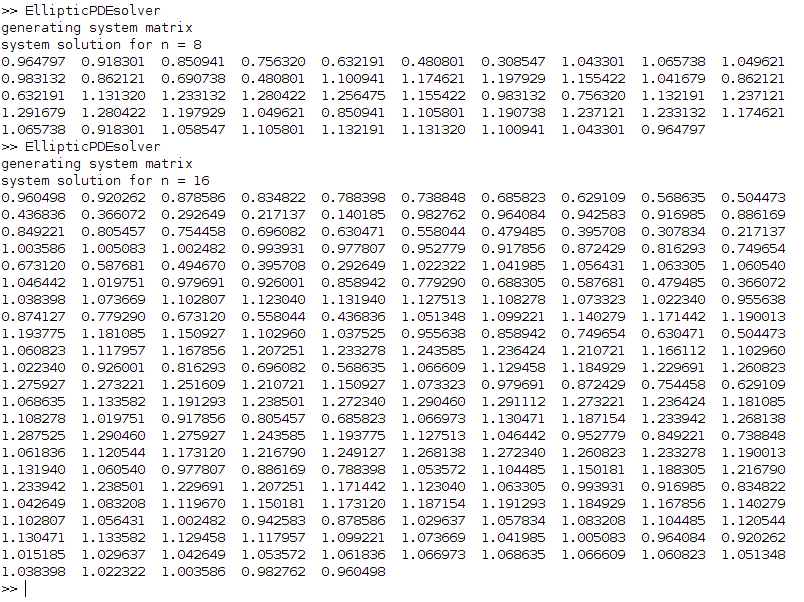
\includegraphics[scale=0.5]{images/img_prob_6_sol_n_8_16.png}
	\caption{Solución del sistema para $n=8$ y $n=16$}
	\label{fig:img_pecc}
\end{figure}
%%%
\item[$(b)$] Comparar los valores obtenidos en el punto anterior con la solución exacta.
\\
Usando el script podemos obtener las siguientes comparaciones de las soluciones aproximada y exacta.
%
%%Figure-Problem
\begin{figure}[H]
	\centering
	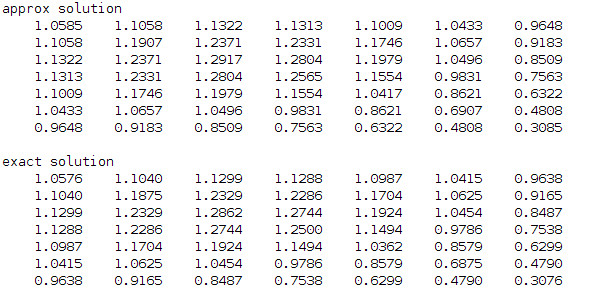
\includegraphics[scale=0.5]{images/img_prob_6_comparison_n8.jpg}
	\caption{Comparación de las soluciones aproximada y exacta para $n=8$}
	\label{fig:img_pecc}
\end{figure}
%%%
%
%%Figure-Problem
\begin{figure}[H]
	\centering
	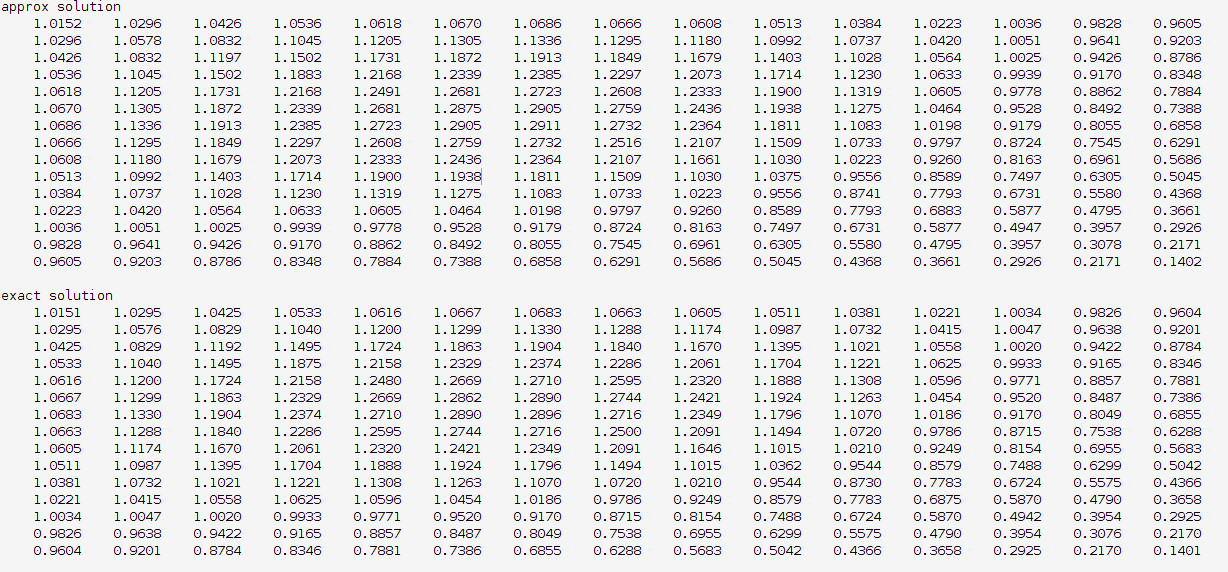
\includegraphics[scale=0.35]{images/img_prob_6_comparison_n16.jpg}
	\caption{Comparación de las soluciones aproximada y exacta para $n=16$}
	\label{fig:img_pecc}
\end{figure}
%%%
%
%%Figure-Problem
\begin{figure}[H]
	\centering
	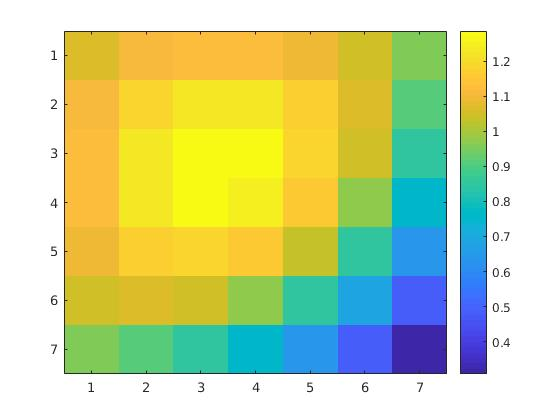
\includegraphics[scale=0.35]{images/img_prob_6_colormap_n8_exact.jpg}
	\caption{Heatmap de la solución exacta para $n=8$}
	\label{fig:img_pecc}
\end{figure}
%%%
%
%%Figure-Problem
\begin{figure}[H]
	\centering
	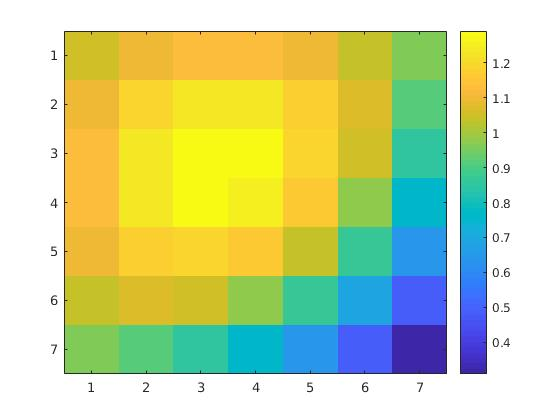
\includegraphics[scale=0.35]{images/img_prob_6_colormap_n8_approx.jpg}
	\caption{Heatmap de la solución aproximada para $n=8$}
	\label{fig:img_pecc}
\end{figure}
%%%
%
%%Figure-Problem
\begin{figure}[H]
	\centering
	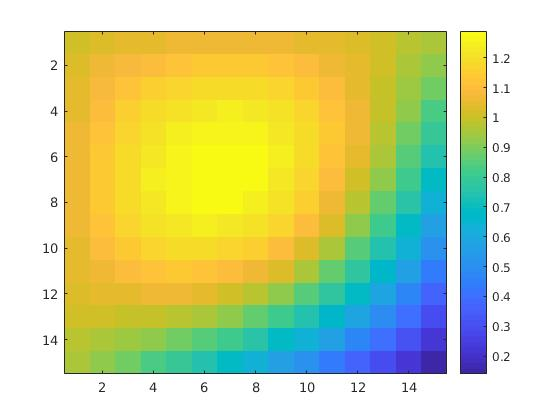
\includegraphics[scale=0.35]{images/img_prob_6_colormap_n16_exact.jpg}
	\caption{Heatmap de la solución exacta para $n=16$}
	\label{fig:img_pecc}
\end{figure}
%%%
%
%%Figure-Problem
\begin{figure}[H]
	\centering
	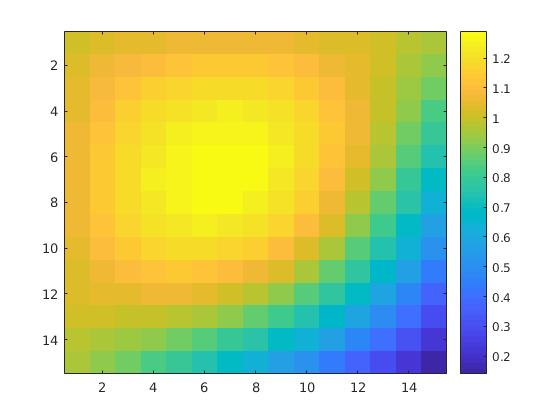
\includegraphics[scale=0.35]{images/img_prob_6_colormap_n16_approx.jpg}
	\caption{Heatmap de la solución aproximada para $n=16$}
	\label{fig:img_pecc}
\end{figure}
%%%
Como se puede observar de las comparaciones, el método devuelve buenas aproximaciones tanto para $n=8$ como para $n=16$.

\item[$(c)$] Defina el sistema lineal resultante al aplicar el metodo de elementos finitos en la solución del problema del valor de frontera de 2 puntos: $-2u''+3u=x^2$, $0\leq x\leq 1$, $u(0)=u(1)=0$,usando malla uniforme y funciones basicas $\phi_j(x)$ como en el libro.\\

\textbf{\underline{Solución:}}

El problema hace referencia a una aproximación por elementos finitos en un entorno 1D tal como se observa en la imagen \ref{2p_mef}.
%%%
%
%%Figure-Problem
\begin{figure}[H]
	\centering
	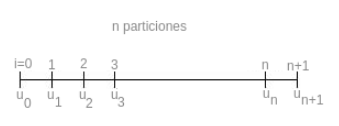
\includegraphics[scale=0.6]{images/2p_bound.png}
	\caption{Representación del problema}
	\label{2p_mef}
\end{figure}
%%%
En el problema se indica las condiciones de frontera en $u_0=0$ y $u_{n+1}=0$. Definiendo sobre el resto de puntos la ecuación usando la aproximación de la derivada  $u''_i=u_{i+1}-2u_i+u_{i-1}$ obtenemos:\\
$$-2.(u_{i+1}-2u_i+u_{i-1})+3u_i=(i/n)^2$$
$$-2.u_{i+1}+7.u_i-2.u_{i-1}=(i/n)^2$$
Remplazando para $i=1,\dots,n$:
$$i=1\to -2u_2+7u_1-2u_0=(1/n)^2$$
$$i=2\to -2u_3+7u_2-2u_1=(2/n)^2$$
$$i=3\to -2u_4+7u_3-2u_2=(3/n)^2$$
$$\vdots$$
$$i=n\to -2u_{n+1}+7u_n-2u_{n-1}=(n/n)^2$$

Usando las ecuaciones de frontera $u_0=0$ y $u_{n+1}=0$ tenemos la forma matricial:\\
\begin{gather*}
\begin{bmatrix}
       7 & -2 & 0 & 0 & \dots & 0 & 0 \\
       -2 & 7 & -2 & 0 & \dots & 0 & 0 \\
       0 & -2 & 7 & -2 & \dots & 0 & 0 \\
       0 & 0 & -2 & 7 & \dots & 0 & 0 \\
       \vdots & \vdots & \vdots & \vdots & \ddots & \vdots & \vdots \\
       0 & 0 & 0 & 0 & \dots & 7 & -2 \\
       0 & 0 & 0 & 0 & \dots & -2 & 7 \\
\end{bmatrix}.
\begin{bmatrix}
    u_1 \\
    u_2 \\
    u_3 \\
    u_4 \\
    \vdots \\
    u_{n-1} \\
    u_n \\
\end{bmatrix}
 = \frac{1}{n^2}.
\begin{bmatrix}
    1^2 \\
    2^2 \\
    3^2 \\
    4^2 \\
    \vdots \\
    (n-1)^2 \\
    n^2 \\
\end{bmatrix}
\end{gather*}



\end{itemize}